\documentclass[tikz,border=1pt]{standalone}
\usepackage[T1]{fontenc}
\usepackage{times}
\usepackage{amsmath,amssymb}
\usepackage{xcolor}
\usetikzlibrary{arrows.meta,positioning,shapes.geometric,calc}

% Exact sampled color palette matching reference image
\definecolor{stage1bg}{HTML}{EBF5FD}
\definecolor{stage1border}{HTML}{5C7997}
\definecolor{stage1cardbg}{HTML}{F6FAFE}

\definecolor{stage2bg}{HTML}{E2F3DF}
\definecolor{stage2border}{HTML}{4E8E53}

\definecolor{stage3bg}{HTML}{FDF6DD}
\definecolor{stage3border}{HTML}{B09455}
\definecolor{stage3cardbg}{HTML}{FFFDF6}

\definecolor{stage4bg}{HTML}{E2DEFC}
\definecolor{stage4border}{HTML}{786A9D}

\definecolor{stage5bg}{HTML}{FDE1EE}
\definecolor{stage5border}{HTML}{D1729A}
\definecolor{stage5cardbg}{HTML}{FFF7FB}

\definecolor{stage6bg}{HTML}{CEE4CF}
\definecolor{stage6border}{HTML}{396740}
\definecolor{stage6cardbg}{HTML}{F2FAF2}

\begin{document}
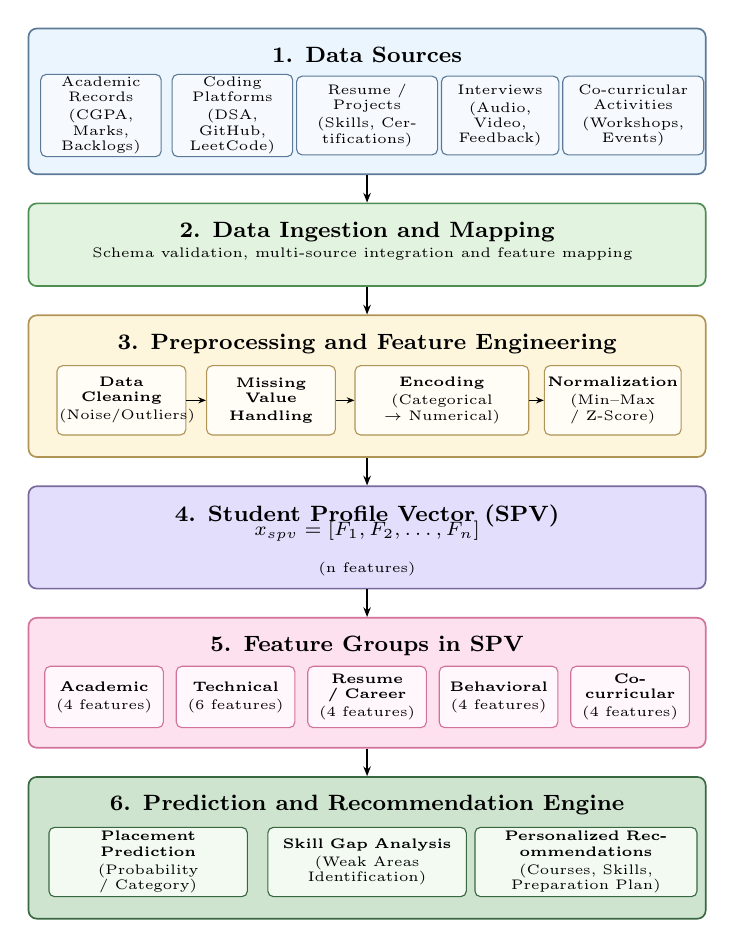
\begin{tikzpicture}[
    >=Stealth,
    outerbox/.style={
        rectangle, rounded corners=3pt, line width=0.6pt,
        inner sep=0pt
    },
    title/.style={
        font=\fontsize{7.8pt}{9.2pt}\selectfont\bfseries, text=black
    },
    arrowdown/.style={
        -{Stealth[length=3.5pt, width=2.7pt]}, line width=0.85pt, draw=black
    }
]

\def\W{86mm}

% ==================== STAGE 1 ====================
\node[outerbox, fill=stage1bg, draw=stage1border, minimum width=\W, minimum height=18.5mm] (c1) at (0, 0) {};
\node[title] at (c1.north) [below=1.2mm] {1. Data Sources};

\begin{scope}[
    every node/.style={
        rectangle, rounded corners=2pt,
        fill=stage1cardbg, draw=stage1border, line width=0.4pt,
        minimum height=10.0mm, align=center,
        inner sep=1.0pt, font=\fontsize{4.6pt}{5.5pt}\selectfont,
        text=black
    }
]
    \node[text width=14.6mm] (s1) at (-33.8mm, -1.8mm) {Academic Records\\[1pt](CGPA, Marks,\\Backlogs)};
    \node[text width=14.6mm] (s2) at (-17.1mm, -1.8mm) {Coding Platforms\\[1pt](DSA, GitHub,\\LeetCode)};
    \node[text width=17.2mm] (s3) at (0.0mm, -1.8mm)    {Resume / Projects\\[1pt](Skills, Certifications)};
    \node[text width=14.2mm] (s4) at (+16.9mm, -1.8mm) {Interviews\\[1pt](Audio, Video,\\Feedback)};
    \node[text width=17.2mm] (s5) at (+33.8mm, -1.8mm) {Co-curricular Activities\\[1pt](Workshops, Events)};
\end{scope}

% ==================== STAGE 2 ====================
\node[outerbox, fill=stage2bg, draw=stage2border, minimum width=\W, minimum height=10.5mm, below=3.5mm of c1] (c2) {};
\node[title] at (c2.north) [below=1.2mm] {2. Data Ingestion and Mapping};
\node[align=center] at (c2.center) [yshift=-1.2mm] {
    {\fontsize{5.4pt}{6.6pt}\selectfont Schema validation, multi-source integration and feature mapping}
};

% ==================== STAGE 3 ====================
\node[outerbox, fill=stage3bg, draw=stage3border, minimum width=\W, minimum height=18.0mm, below=3.5mm of c2] (c3) {};
\node[title] at (c3.north) [below=1.2mm] {3. Preprocessing and Feature Engineering};

\begin{scope}[
    card3/.style={
        rectangle, rounded corners=2pt,
        fill=stage3cardbg, draw=stage3border, line width=0.4pt,
        minimum height=8.8mm, align=center,
        inner sep=0.8pt, font=\fontsize{4.6pt}{5.5pt}\selectfont,
        text=black
    }
]
    \node[card3, text width=15.8mm] (p1) at ($(c3.center) + (-31.2mm, -1.8mm)$) {\textbf{Data Cleaning}\\[1pt](Noise/Outliers)};
    \node[card3, text width=15.8mm] (p2) at ($(c3.center) + (-12.2mm, -1.8mm)$) {\textbf{Missing Value}\\[1pt]\textbf{Handling}};
    \node[card3, text width=21.5mm] (p3) at ($(c3.center) + (+9.5mm,  -1.8mm)$) {\textbf{Encoding}\\[1pt](Categorical $\rightarrow$ Numerical)};
    \node[card3, text width=16.8mm] (p4) at ($(c3.center) + (+31.2mm, -1.8mm)$) {\textbf{Normalization}\\[1pt](Min--Max / Z-Score)};
    
    \draw[-{Stealth[length=2.8pt, width=2.2pt]}, line width=0.55pt, draw=black] (p1.east) -- (p2.west);
    \draw[-{Stealth[length=2.8pt, width=2.2pt]}, line width=0.55pt, draw=black] (p2.east) -- (p3.west);
    \draw[-{Stealth[length=2.8pt, width=2.2pt]}, line width=0.55pt, draw=black] (p3.east) -- (p4.west);
\end{scope}

% ==================== STAGE 4 ====================
\node[outerbox, fill=stage4bg, draw=stage4border, minimum width=\W, minimum height=13.0mm, below=3.5mm of c3] (c4) {};
\node[title] at (c4.north) [below=1.2mm] {4. Student Profile Vector (SPV)};
\node[align=center] at (c4.center) [yshift=-1.4mm] {
    {\fontsize{6.8pt}{8.2pt}\selectfont $x_{spv} = [F_1, F_2, \dots, F_n]$}\\[1.2pt]
    {\fontsize{5.0pt}{6.2pt}\selectfont (n features)}
};

% ==================== STAGE 5 ====================
\node[outerbox, fill=stage5bg, draw=stage5border, minimum width=\W, minimum height=16.5mm, below=3.5mm of c4] (c5) {};
\node[title] at (c5.north) [below=1.2mm] {5. Feature Groups in SPV};

\begin{scope}[
    every node/.style={
        rectangle, rounded corners=2pt,
        fill=stage5cardbg, draw=stage5border, line width=0.4pt,
        minimum height=7.8mm, align=center,
        inner sep=0.8pt, font=\fontsize{4.6pt}{5.5pt}\selectfont,
        text width=14.5mm, text=black
    }
]
    \node (f1) at ($(c5.center) + (-33.4mm, -1.8mm)$) {\textbf{Academic}\\[1pt](4 features)};
    \node (f2) at ($(c5.center) + (-16.7mm, -1.8mm)$) {\textbf{Technical}\\[1pt](6 features)};
    \node (f3) at ($(c5.center) + (0.0mm,   -1.8mm)$) {\textbf{Resume / Career}\\[1pt](4 features)};
    \node (f4) at ($(c5.center) + (+16.7mm, -1.8mm)$) {\textbf{Behavioral}\\[1pt](4 features)};
    \node (f5) at ($(c5.center) + (+33.4mm, -1.8mm)$) {\textbf{Co-curricular}\\[1pt](4 features)};
\end{scope}

% ==================== STAGE 6 ====================
\node[outerbox, fill=stage6bg, draw=stage6border, minimum width=\W, minimum height=18.0mm, below=3.5mm of c5] (c6) {};
\node[title] at (c6.north) [below=1.2mm] {6. Prediction and Recommendation Engine};

\begin{scope}[
    every node/.style={
        rectangle, rounded corners=2pt,
        fill=stage6cardbg, draw=stage6border, line width=0.4pt,
        minimum height=8.8mm, align=center,
        inner sep=1.0pt, font=\fontsize{4.6pt}{5.5pt}\selectfont,
        text=black
    }
]
    \node[text width=24.5mm] (r1) at ($(c6.center) + (-27.8mm, -1.8mm)$) {\textbf{Placement Prediction}\\[1pt](Probability / Category)};
    \node[text width=24.5mm] (r2) at ($(c6.center) + (0.0mm,   -1.8mm)$) {\textbf{Skill Gap Analysis}\\[1pt](Weak Areas Identification)};
    \node[text width=27.5mm] (r3) at ($(c6.center) + (+27.8mm, -1.8mm)$) {\textbf{Personalized Recommendations}\\[1pt](Courses, Skills, Preparation Plan)};
\end{scope}

% ==================== VERTICAL CONNECTING ARROWS ====================
\draw[arrowdown] (c1.south) -- (c2.north);
\draw[arrowdown] (c2.south) -- (c3.north);
\draw[arrowdown] (c3.south) -- (c4.north);
\draw[arrowdown] (c4.south) -- (c5.north);
\draw[arrowdown] (c5.south) -- (c6.north);

\end{tikzpicture}
\end{document}
